\section{Worked example: the heat equation}\label{m:sec:heat}

Chapters~\ref{ch:manifold} to~\ref{ch:generators} state the method, generative Bayesian computation (GBC), and its theory for a general evolution equation. This chapter puts three equations through them and asks what the theorems say about each and what an implementation delivers. It assumes from Chapter~\ref{ch:manifold} the observation model, the Bernstein von Mises theorems of Nickl and of Konen and Nickl with Conditions 1 and 2 of Nickl on the prior and the forward map, and Algorithm~\ref{m:alg:gbc}; from Chapter~\ref{ch:adjoint} the adjoint summary and the dimension $J_N$ that the theory licenses for it; and from Chapter~\ref{ch:generators} the transfer theorem, the accuracy it asks of a generator, and the localized training of Algorithm~\ref{m:alg:loc}. A result there that is conditional on Assumption~\ref{m:ass:U} or Assumption~\ref{m:ass:u2p} is conditional here in the same way: the first is open (Open Question~\ref{m:op:unif}), and the second holds in the setting of Theorem~\ref{m:thm:u2ploc}.

The heat equation comes first because every object in it is explicit. Two dimensional Navier Stokes about the Taylor Green vortex adds the nonlinearity as a compact correction to the heat equation case. The Schr\"odinger equation removes the dissipation, and with it the smoothing on which the supremum norm theorems rest. The last two sections connect the construction to earlier methods that share its structure and to the sixth problem, and list five questions that remain open. Except where a result is attributed, the computations and experiments are ours, and the Notes at the end say which results are quoted and which are, to our knowledge, new.

Let $\Omega=\T^d$, $\partial_tu=\nu\Delta u$, $u(0)=\theta$, so that $u_\theta(t,x)=\sum_j e^{-\nu\lambda_jt}\theta_je_j(x)$ with $\lambda_j=4\pi^2|k_j|^2$. Take the prior $\theta_j\sim N(0,\rho^2\lambda_j^{-\alpha})$ independently, truncated to $|k|\le K_{\max}$, and observations \eqref{m:eq:model} with $t_i\sim\mathrm{Unif}[T_0,T]$, $x_i\sim\mathrm{Unif}(\T^d)$.

\subsubsection{Exact posterior and sufficient statistic} By \eqref{m:eq:linpost}, the posterior is $N(m_N,V_N)$ with $V_N^{-1}=\Phi^\top\Phi+\rho^{-2}\Lambda^\alpha$, and the sufficient statistic is $S_N=\Phi^\top Y$, i.e.\ $S_{N,j}=\sum_ie^{-\nu\lambda_jt_i}e_j(x_i)Y_i$: the data projected onto mode $j$ and propagated backward by the (self adjoint) heat semigroup to time zero.

\subsubsection{Information per mode and the dissipation barrier} By \eqref{m:eq:gram},
\begin{equation}\label{m:eq:iota}
\begin{aligned}
\frac1N\Phi^\top\Phi&\to\diag(\iota_j),\\
\iota_j(T_0)&=\frac{1}{T-T_0}\int_{T_0}^Te^{-2\nu\lambda_jt}dt\\
&=\frac{e^{-2\nu\lambda_jT_0}\big(1-e^{-2\nu\lambda_j(T-T_0)}\big)}{2\nu\lambda_j(T-T_0)} .
\end{aligned}
\end{equation}
With $T_0=0$, $\iota_j\asymp(2\nu\lambda_jT)^{-1}$ decays polynomially in $j$; with $T_0>0$ the factor $e^{-2\nu\lambda_jT_0}$ makes it decay exponentially in $|k_j|^2$. Table~\ref{m:tab:iota} gives the values and Figure~\ref{m:fig:heat}(left) plots them. At $|k|=16$ the information drops by a factor of about $2\times10^4$ when the first observation is delayed to $T_0=0.05$, and by about $10^{17}$ at $T_0=0.2$. This is the mechanism of the inverse logarithmic lower bound in Theorem~4 of Nickl and Titi~\cite{nickltiti2024}, as a table: a mode that has decayed by $e^{-\nu\lambda_jT_0}$ before the first observation is recoverable only with about $e^{2\nu\lambda_jT_0}$ times more data, the square of that factor, since the information a mode carries scales with the square of its amplitude. It is also the viscous curse in the computation of Nickl and Wang~\cite{nicklwang2024} (Section~\ref{sec:gradstab}). Were their remaining conditions to carry over, the curvature constant $c_{\min}$ of their localized Langevin algorithm would be $\min_j\iota_j$, which Section~\ref{m:sec:nondiss} contrasts with the dispersive case, where it is one uniformly.

\begin{table}[t]\centering\small
\caption{Per mode information $\iota_k(T_0)$ for the two dimensional heat equation, $\nu=0.01$, $T=1$, mode $k=(|k|,0)$. Here $T_0$ is the time at which observation begins, so that $T_0=0$ is the design of \eqref{m:eq:model} and $T_0>0$ delays the start; the closed form is \eqref{m:eq:iota}.}\label{m:tab:iota}
\begin{tabular}{rllll}
\toprule
$|k|$ & $\iota_k(0)$ & $\iota_k(0.05)$ & $\iota_k(0.2)$ & $1/\iota_k(0)=\sigma_k^2$\\
\midrule
1 & $6.91\times10^{-1}$ & $6.76\times10^{-1}$ & $6.33\times10^{-1}$ & $1.45$\\
2 & $3.03\times10^{-1}$ & $2.70\times10^{-1}$ & $1.94\times10^{-1}$ & $3.30$\\
4 & $7.92\times10^{-2}$ & $4.43\times10^{-2}$ & $7.91\times10^{-3}$ & $12.6$\\
8 & $1.98\times10^{-2}$ & $1.66\times10^{-3}$ & $1.01\times10^{-6}$ & $50.5$\\
16 & $4.95\times10^{-3}$ & $2.13\times10^{-7}$ & $1.72\times10^{-20}$ & $202$\\
32 & $1.24\times10^{-3}$ & $3.61\times10^{-21}$ & $9.17\times10^{-74}$ & $809$\\
\bottomrule
\end{tabular}
\end{table}

\begin{figure}[tp]\centering
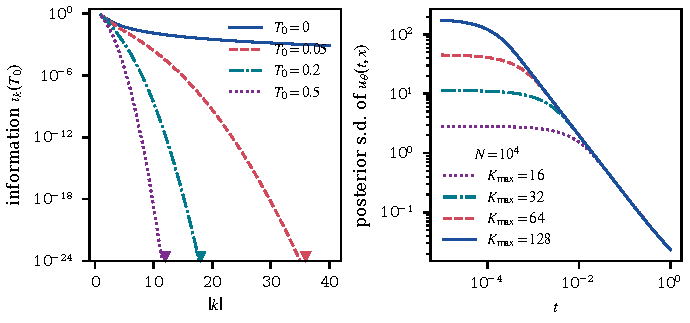
\includegraphics[width=\textwidth]{mf_heat}
\caption{Left: per mode information $\iota_k(T_0)$ from \eqref{m:eq:iota} for the two dimensional heat (Stokes) equation, $\nu=0.01$, $T=1$, for four observation start times; a triangle marks where a curve falls below $10^{-24}$ and leaves the frame. Right: posterior standard deviation of $u_\theta(t,x)$ at a fixed point, $\sqrt{\sum_{0<|k|\le K_{\max}}e^{-2\nu\lambda_kt}/(N\iota_k)}$ with $\iota_k=\iota_k(0)$, as a function of $t$ for $N=10^4$ and four truncations, $K_{\max}=16,32,64,128$. The $1/\sqrt N$ scaling is exact. At each fixed truncation the sum is finite at $t=0$ and the curve ends in a plateau, which rises by a factor close to four each time $K_{\max}$ doubles and so grows without bound with the truncation: this divergence as $t\to0$ is the failure of the supremum norm Bernstein von Mises theorem at the initial time. For larger $t$ the curves coincide, and the finiteness of the sum there whatever the truncation is parabolic smoothing.}\label{m:fig:heat}
\end{figure}

\begin{proposition}[Gram concentration and the finite $N$ Bernstein von Mises error]\label{m:prop:gram}
Let $\Phi$ be the design matrix \eqref{m:eq:design} for the heat equation with $D$ modes, uniform design on $[0,T]\times\T^d$, and $\norm{e_j}_\infty\le\sqrt2$, and let $N\ge D\log D$. Then, with the absolute constant $c=12$,
\[
\begin{gathered}
\Big\|\frac1N\Phi^\top\Phi-\diag(\iota_j)\Big\|_{op}\le c\,\sqrt{\frac{D\log D}{N}}\\
\text{with probability at least }1-D^{-1},
\end{gathered}
\]
and consequently, if $c\sqrt{D\log D/N}<\min_j\iota_j$, for the exact posterior covariance $V_N=(\Phi^\top\Phi+\Sigma_0^{-1})^{-1}$ and its Bernstein von Mises prediction $\bar V_N=(N\diag(\iota_j)+\Sigma_0^{-1})^{-1}$,
\[
\begin{gathered}
\norm{NV_N-N\bar V_N}_{op}\le\frac{c\sqrt{D\log D/N}}{\min_j\iota_j\,(\min_j\iota_j-c\sqrt{D\log D/N})}\\
\text{on the same event.}
\end{gathered}
\]
\end{proposition}

\begin{proof}
$\frac1N\Phi^\top\Phi=\frac1N\sum_i\phi_i\phi_i^\top$ with $\phi_i=(s_j(t_i)e_j(x_i))_j$ i.i.d., $E\phi_i\phi_i^\top=\diag(\iota_j)$ by orthonormality of $(e_j)$ and \eqref{m:eq:iota}, and $\norm{\phi_i}^2\le2D$. The matrix Bernstein inequality~\cite[Theorem 6.1.1]{tropp2015}, applied to the centered summands $(\phi_i\phi_i^\top-\diag(\iota_j))/N$, whose operator norms are at most $L=4D/N$ and whose variance proxy is at most $v=2D\max_j\iota_j/N\le2D/N$, bounds the probability that $\norm{N^{-1}\Phi^\top\Phi-\diag(\iota_j)}_{op}\ge t$ by $2D\exp\{-(t^2/2)/(v+Lt/3)\}$. At $t=\frac23\ell L+\sqrt{2\ell v}$ with $\ell=\log(2D^2)$ the exponent is at least $\ell$, so this probability is at most $D^{-1}$. For $D\ge2$, $\ell\le3\log D$, hence $t\le8D\log D/N+\sqrt{12D\log D/N}\le(8+\sqrt{12})\sqrt{D\log D/N}<12\sqrt{D\log D/N}$, where the middle step uses $D\log D/N\le1$; for $D=1$ the probability claimed is $0$ and there is nothing to prove. The second follows from the resolvent identity $NV_N-N\bar V_N=N\bar V_N(N\diag\iota-\Phi^\top\Phi)V_N$ and $\norm{N\bar V_N}_{op}\le1/\min_j\iota_j$, $\norm{NV_N}_{op}\le(\min_j\iota_j-c\sqrt{D\log D/N})^{-1}$.
\end{proof}

Since $\min_{j\le D}\iota_j\asymp D^{-2/d}$ by \eqref{m:eq:iota}, the relative error of the Bernstein von Mises covariance is $O(D^{2/d}\sqrt{D\log D/N})$, which is small exactly when $D\ll N^{d/(d+4)}$ up to logarithms. This is a quantitative counterpart, for the linear problem, of the dimension $J_N\asymp N^{d/(2\gamma+d)}$ of the projection $p_N$ in Nickl's centering \eqref{m:eq:thetahat} (his prior \eqref{m:eq:prior} is not truncated, and Condition~1 of Nickl~\cite{nicklbvm2024} imposes no dimension constraint).

\subsubsection{The Bernstein von Mises theorem, checked at finite $N$} Theorem~\ref{m:thm:nickl2} predicts that the posterior on mode $j$ is asymptotically $N(\tilde\theta_j,\sigma_j^2/N)$ with $\sigma_j^2=1/\iota_j$, and more precisely, keeping the prior term, with variance $(N\iota_j+\rho^{-2}\lambda_j^\alpha)^{-1}$. Figure~\ref{m:fig:heatgbc} compares this with the exact posterior from \eqref{m:eq:linpost} for the fixed truth $\theta_{0,k}=(1+k^2)^{-1}\mathrm{sign}(\sin k)$: the maximal relative discrepancy between the exact and the asymptotic standard deviation is $1.4\times10^{-4}$. The limit $\Ncal_{\theta_0}$ has variance $\sigma_j^2\asymp2\nu\lambda_jT$ growing with $j$, so $\sum_j\lambda_j^{-a}\sigma_j^2<\infty$ exactly when $a>1+d/2$, which is the tightness range of Proposition~2 of Nickl~\cite{nicklbvm2024}; the Gaussian limit is white noise roughened by $(-\Delta)^{1/2}$, and lives in $H^{-a}$ but not in $L^2$.

\begin{figure}[tp]\centering
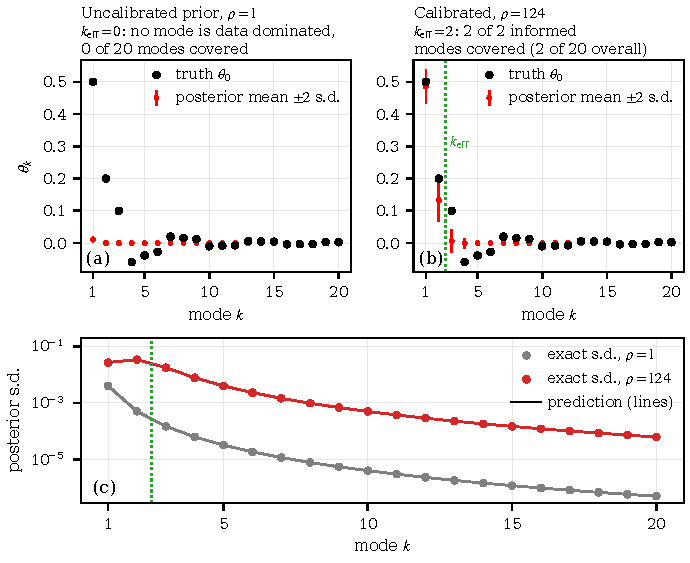
\includegraphics[width=\textwidth]{mf_heat_gbc}
\caption{Heat equation on $\T^1$, $N=2000$ observations, $K_{\max}=20$, $\alpha=3$, $\nu=0.01$, with the exact posterior of \eqref{m:eq:linpost}. Panel (a): the uncalibrated prior, $\rho=1$. No mode is data dominated, $k_{\rm eff}=0$; the truth lies up to $4949$ prior standard deviations from the prior mean and outside a two standard deviation credible interval in all $20$ modes. Panel (b): the same data with $\rho$ calibrated so that the prior standard deviation at $|k|=1$ matches the initial condition, $\rho=124$. Now $k_{\rm eff}=2$, and the truth lies inside the interval in every informed mode, with largest standardized error $1.96$. Panel (c): exact posterior standard deviation per mode in both settings against the prediction $(N\iota_k+\rho^{-2}\lambda_k^\alpha)^{-1/2}$ (lines). The agreement is close in both, which is why it validates nothing for $\rho=1$. Section~\ref{m:sec:expfinite} gives the diagnosis and Section~\ref{m:sec:covstudy} the coverage over replicates.}\label{m:fig:heatgbc}
\end{figure}

\subsubsection{Forward simulation and the trajectory theorem} Pushing the posterior through the heat flow gives $u_\theta(t,x)\mid Z\sim N\big(\sum_je^{-\nu\lambda_jt}\tilde\theta_je_j(x),\ \sum_{j,l}e^{-\nu(\lambda_j+\lambda_l)t}(V_N)_{jl}e_j(x)e_l(x)\big)$. Keeping only the diagonal terms, which is justified asymptotically because $\frac1N\Phi^\top\Phi$ concentrates on $\diag(\iota_j)$ by Proposition~\ref{m:prop:gram}, the posterior standard deviation of the state at time $t$ is, asymptotically, $N^{-1/2}\big(\sum_je^{-2\nu\lambda_jt}\sigma_j^2e_j(x)^2\big)^{1/2}$. Since $\sigma_j^2\asymp\lambda_j$, the series $\sum_j\lambda_je^{-2\nu\lambda_jt}$ converges for every $t>0$ and diverges at $t=0$: the trajectory is $\sqrt N$ estimable in supremum norm at every positive time, and the initial condition is not. Figure~\ref{m:fig:heat}(right) shows this, which is Theorem~\ref{m:thm:nickl1} and Remark~3 of Nickl~\cite{nicklbvm2024} in one picture; it is also Corollary~\ref{m:cor:commute}, since for a linear equation solve then simulate and simulate the limit are the same operation.

\subsubsection{GBC for the heat equation} Algorithm~\ref{m:alg:gbc} with the preconditioned summary $\tilde S_N=V_N\Phi^\top Y$ of Proposition~\ref{m:prop:linsuff} and an identity plus scale generator is exact. The learning problem has $D$ slopes (all equal to one), $D$ intercepts (all zero) and a $D\times D$ scale; with the prior diagonal and the Gram matrix asymptotically diagonal, the scale is asymptotically diagonal with entries $(N\iota_j+\rho^{-2}\lambda_j^\alpha)^{-1/2}$, so a generator with an identity skip, which fixes the slopes, and $2D$ free parameters, the intercepts and the diagonal of the scale, suffices, and $M\gg D$ simulations estimate it. This is the baseline against which the nonlinear case should be measured: the cost of nonlinearity is exactly the cost of the compact perturbation $\Kcal$ in \eqref{m:eq:fredholm}.

\subsection{The resolution the data support}\label{m:sec:resolution}

Four truncation dimensions appear in this part and they are different objects, so we fix them here once, in Table~\ref{m:tab:dims}.

\begin{table}[t]\centering\small
\caption{The four truncation dimensions, with the values they take in the computations of this part. The last column reports what is actually used, over $N=10^3$ to $1.3\times10^6$ where a range is given.}\label{m:tab:dims}
\begin{tabular}{@{}l>{\raggedright\arraybackslash}p{1.35in}>{\raggedright\arraybackslash}p{1.5in}l@{}}
\toprule
Symbol & What it is & Set by & Here\\
\midrule
$J_N$ & summary dimension the theory licenses & $N^{d/(2\gamma+d)}$, Theorem~\ref{m:thm:nickl2} & $2$ to $3$\\
$k_{\rm eff}$ & highest mode the data dominate the prior on & $N\iota_k\ge\rho^{-2}\lambda_k^\alpha$ & $0$ to $5$\\
$K_{\max}$ & modes retained in a computation & the user, $\ge k_{\rm eff}$ & $8$ to $128$\\
$D$ & coefficients the generator outputs & $\#\{|k|\le K_{\max}\}$ & $6$ to $20$\\
\bottomrule
\end{tabular}
\end{table}

\noindent Only $J_N$, and for the heat equation $D$ (Proposition~\ref{m:prop:regfixed}), carry asymptotic guarantees; $k_{\rm eff}$ is a property of the experiment and of the prior, computed in \eqref{m:eq:jeffdata} below and reported for each run in Section~\ref{m:sec:experiments}; $K_{\max}$ and $D$ are choices, and the rest of this subsection argues that taking them well above $J_N$ costs nothing and is what one should do. The $k_{\rm eff}$ range is $0$ at the uncalibrated prior of Figure~\ref{m:fig:heatgbc} and $2$ to $5$ at the calibrated one, whose $K_{\max}$ is $20$; Section~\ref{m:sec:expstudy} has $K_{\max}=D=8$ and Section~\ref{m:sec:expns} has $D=6$, and the analytic computation of Figure~\ref{m:fig:heat}(right) takes $K_{\max}$ from $16$ to $128$.

The theory licenses a summary of dimension $J_N\asymp N^{d/(2\gamma+d)}$. With the regularity $\gamma>12$ that Konen and Nickl~\cite{konennickl2026} require and $d=2$ this is at most $N^{1/13}$, its value at $\gamma=12$: at most $1.7$ modes at $N=10^3$, $2.9$ at $N=10^6$, $5.9$ at $N=10^{10}$. Table~\ref{m:tab:iota} tabulates $\iota_j$ to $|k|=32$ and Figure~\ref{m:fig:heat} plots to $|k|=40$.

Ask independently how many modes the data inform, with no reference to the asymptotic theory. A mode is informed when its data precision exceeds its prior precision, $N\iota_k\ge\rho^{-2}\lambda_k^\alpha$. Using $\iota_k=(1-e^{-2\nu\lambda_kT})/(2\nu\lambda_kT)\sim(2\nu\lambda_kT)^{-1}$ for $\nu\lambda_kT\gg1$, the crossover sits at $\lambda_K=(N\rho^2/2\nu T)^{1/(\alpha+1)}$, and since $\#\{k:\lambda_k\le\Lambda\}\asymp\Lambda^{d/2}$ the number of informed modes is
\begin{equation}\label{m:eq:jeffdata}
J^{\rm data}_N\asymp\Big(\frac{N\rho^2}{2\nu T}\Big)^{d/(2(\alpha+1))}.
\end{equation}
The fixed prior of Section~\ref{m:sec:heat} has covariance eigenvalues $\rho^2\lambda_j^{-\alpha}$ on the modes with $|k|\le K_{\max}$, and the series it truncates has reproducing kernel Hilbert space (RKHS) $H^\alpha_0$, the RKHS of \eqref{m:eq:prior} when $\gamma=\alpha$; under \eqref{m:eq:prior} itself, whose scale $\rho^2=1/(N\delta_N^2)$ shrinks with $N$, the informed count is instead $J^{\rm eff}_N=o(J_N)$ (Proposition~\ref{m:prop:pr} and Remark~\ref{m:rem:jeff}). Comparing exponents,
\[
\frac{d}{2\gamma+d}\quad\text{against}\quad\frac{d}{2(\alpha+1)},
\]
which are equal precisely when $2(\alpha+1)=2\alpha+d$, that is when $d=2$, the case the framework is built for. In $d=1$ and $d=3$ the exponents differ, but only slightly: $1/7$ against $1/8$ and $1/3$ against $3/8$ at $\alpha=\gamma=3$, so that, constants aside, the two dimensions differ by the slowly growing factors $N^{1/56}$ and $N^{1/24}$, and the numerical gap over seven decades of $N$ is a factor between $1.1$ and $2.6$. Solving $N\iota_k=\rho^{-2}\lambda_k^\alpha$ numerically for $d=1$, $\alpha=3$, with $\rho$ calibrated so the prior standard deviation at $k=1$ matches the initial condition, gives $J^{\rm data}_N=2,2,3,4,6,8,11,15$ at $N=10^3,\dots,10^{10}$ and a fitted exponent of $0.134$ against the $0.125$ that \eqref{m:eq:jeffdata} predicts; the excess is the integer rounding of a mode count, which biases the slope upward at small counts. Read the other way, seven decades of data buy a factor of $7.5$ in resolution.

So $J_N$ is not a conservative artifact of the proof. It is the number of modes the experiment resolves, and any procedure that respects this prior, on this observation model, resolves the same number. What makes it small is the regularity the framework demands: $\gamma>12$ is a very smooth prior, and a very smooth prior leaves few modes in which the data outweigh it. Relaxing that regularity requirement, which is open, would raise the licensed and the achievable resolution together.

Table~\ref{m:tab:iota} and Figure~\ref{m:fig:heat} tabulate $\iota_j$ over a wide band because $\iota_j$ is a property of the forward operator, defined at every mode and worth displaying precisely to show how fast the barrier bites; they are not claims that those modes are estimable. And the grid on which the forward solve is carried out is a fifth quantity, not one of the four: it must resolve the dynamics rather than the estimand, and is far finer than $K_{\max}$ demands. Where a statement concerns estimability we write $J_N$; where it concerns what the generator outputs we write $D$.

\subsubsection{Which constraint binds} Two questions follow from a $J_N$ this small. First, what the method delivers beyond a Laplace approximation in a handful of modes: at $N=80$, the sample size of the Navier Stokes run, nothing on accuracy (Section~\ref{m:sec:expns}). What is delivered is amortization and simulation only access to the forward map. Second, whether $J_N$ is ever large enough for the condition $M\gg J_N$ of Theorem~\ref{m:thm:qnnA}, which Corollary~\ref{m:cor:locG}(ii) carries over at every localization radius, to bind before $D$ does. Here it is not, by a wide margin: $J_N$ lies between $2$ and $6$, while the experiments use $M$ between $250$ and $32000$, a budget set by the term $a_v\asymp D/M$ of \eqref{m:eq:decomp} and not by $J_N$ at all. For $M=1200$, a value in that range, to bind one needs $J_N\approx1200$, which at $d=2$, $\gamma=12$ arrives at $N\approx10^{40}$. The condition is vacuous under this prior, not vacuous in general: at the $\gamma=3$ Schauder theory is expected to permit (Open Question~\ref{m:op:unif}) the same $J_N$ arrives at $N\approx2\times10^{12}$. Relaxing the regularity requirement is what would make the simulation budget, rather than the dissipation barrier, the thing that limits resolution.

\section{Worked example: two dimensional Navier Stokes}\label{m:sec:ns}

Consider the periodic two dimensional system in the form of Konen and Nickl~\cite{konennickl2026},
\begin{equation}\label{m:eq:nsproj}
\frac{du}{dt}+\nu Au+B[u,u]=f,\qquad u(0)=\theta\in\Hds{\alpha},
\end{equation}
with $A=-\Delta$ on divergence free mean zero fields, whose eigenfunctions are $e_j(x)=c_jh_{k_j}(x)$, $c_j=(-k_{j,2},k_{j,1})/|k_j|$, $h_k=e^{2\pi ik\cdot x}$, with eigenvalues $\lambda_j=4\pi^2|k_j|^2$; one degree of freedom per wavevector because of incompressibility. Two conventions for the torus are used from here on and no formula mixes them: the unit torus, where $\lambda_k=4\pi^2|k|^2$, for the Stokes limit and Figure~\ref{m:fig:tg}, as for the heat equation of Section~\ref{m:sec:heat} and the Schr\"odinger equation of Section~\ref{m:sec:nondiss}, and the $2\pi$ periodic torus, where $\lambda_k=|k|^2$, for the Taylor Green vortex, Remark~\ref{m:rem:advection} and the experiment of Section~\ref{m:sec:expns}; Section~\ref{m:sec:tg} converts between them.

\subsection{The Stokes limit and the linearization}

If $\theta_0=0$ and $f=0$ then $u_{\theta_0}\equiv0$, the linearized equation \eqref{m:eq:tangentgen} is the Stokes equation $\partial_tU+\nu AU=0$, $\I_{\theta_0}=\Lcal$, $\Kcal=0$ in \eqref{m:eq:fredholm}, and Section~\ref{m:sec:heat} applies verbatim with the divergence free basis: the sufficient statistic is the adjoint Stokes flow of the data, the information per mode is \eqref{m:eq:iota}, the Bernstein von Mises covariance is $T(\I^*\I)^{-1}$ with diagonal $1/\iota_j=2\nu\lambda_jT/(1-e^{-2\nu\lambda_jT})$, and the limit $\Ncal_{\theta_0}$ is tight on $\Hds{-\beta}$ for $\beta>2$ (Proposition~2.7 of Konen and Nickl~\cite{konennickl2026}). The RKHS of the limit is $\Hds{-1}$ because $\sigma_j^2\asymp\lambda_j$ means the covariance operator is $\asymp(-\Delta)$, whose RKHS norm is $\norm{\cdot}_{\dot H^{-1}}$.

\subsubsection{The Taylor Green background} To see the nonlinearity we need a background flow about which the linearized equation is tractable. The Taylor Green vortex~\cite{taylorgreen1937} of \eqref{m:eq:tg} below, on the $2\pi$ periodic torus, is an exact solution of \eqref{m:eq:nsproj} with $f=0$, because $(u\cdot\nabla)u$ is a gradient and is absorbed into the pressure; it has wavevectors $(\pm1,\pm1)$ only, and decays at the Stokes rate of its own mode. On this torus $\lambda_k=|k|^2$, so that the mode $(1,1)$ decays at the rate $2\nu$. Take $\theta_0=u_{\rm TG}(0)$ as the true initial condition. The equation linearized at a background $u_\vartheta$ is
\begin{equation}\label{m:eq:tangentgen}
\partial_tU+\nu AU+B[u_\vartheta,U]+B[U,u_\vartheta]=0,\qquad U(0)=h,
\end{equation}
and because $u_{\rm TG}$ has four Fourier modes, $B[u_{\rm TG},\cdot]+B[\cdot,u_{\rm TG}]$ couples wavevector $k$ only to $k\pm(1,\pm1)$. Section~\ref{m:sec:tg} computes that coupling explicitly. The tangent operator is the Stokes diagonal $-\nu|k|^2$ plus a sparse skew coupling to the four diagonal neighbors whose row sum is $\asymp A|k|$, and Remark~\ref{m:rem:advection} measures the ratio of this coupling to the viscous decay.

\begin{remark}[The advection to dissipation ratio, with constants]\label{m:rem:advection}
Form the Jacobian of the vorticity right hand side at $u_{\rm TG}(0)$ on the $2\pi$ torus, where $\lambda_k=|k|^2$, and compare shell by shell the off diagonal row sum of moduli against the diagonal $\nu|k|^2$. The four Taylor Green coefficients have components of modulus $A/4$ and are orthogonal to their own wavevectors, so the transport term $(u_{\rm TG}\cdot\nabla)$ contributes $cA|k|$ to the row sum with $c$ near one, while the stretching term contributes $O(A)$ and is negligible past the first few shells. Measured at $n=48$, $\nu=0.01$, $A=1$, the row sum is $cA|k|$ with $c$ between 0.74 and 0.98 (the 10th and 90th percentiles) over $6\le|k|\le n/3$, median 0.91, so
\[
\frac{\text{advective coupling at }k}{\text{viscous decay at }k}=\frac{cA}{\nu|k|},\qquad
c\approx0.91 .
\]
The measured ratio is 6.2 at $|k|=16$, against 5.7 from this formula; the formula crosses one at $|k|\approx91$ and reaches a tenth only near $|k|\approx910$. Two things follow. The $1/|k|$ decay is what makes $\Kcal$ in \eqref{m:eq:fredholm} compact, so the Fredholm decomposition is meaningful. But the constant $A/\nu$ is large, so at this viscosity the nonlinear correction to the Stokes information operator is of order one across every mode the truncation of Section~\ref{m:sec:expns} resolves: there the Stokes limit is a structural guide, not a numerical approximation. Computed by \texttt{ns/advection\_ratio.py}.
\end{remark}

\subsection{The explicit Taylor Green coupling}\label{m:sec:tg}

The Taylor Green vortex
\begin{equation}\label{m:eq:tg}
u_{\rm TG}(t,x)=A\,e^{-2\nu t}\big(\sin x_1\cos x_2,\ -\cos x_1\sin x_2\big)
\end{equation}
on the $2\pi$ periodic torus has the four Fourier coefficients $\hat u_\ell$, $\ell\in\{(\pm1,\pm1)\}$, each with components of modulus $Ae^{-2\nu t}/4$. With $\widehat{(u\cdot\nabla)v}_k=\sum_{\ell+m=k}i\,(\hat u_\ell\cdot m)\,\hat v_m$ and $P_k=\Id-kk^\top/|k|^2$ the Leray projector in Fourier space, the linear operator in \eqref{m:eq:tangentgen} at $u_\vartheta=u_{\rm TG}$ is
\begin{equation}\label{m:eq:tgcoupling}
\begin{split}
\widehat{\big(B[u_{\rm TG},U]+B[U,u_{\rm TG}]\big)}_k={}&i\,P_k\sum_{\ell\in\{(\pm1,\pm1)\}}\Big[(\hat u_\ell\cdot(k-\ell))\,\hat U_{k-\ell}\\
&\qquad+(\hat U_{k-\ell}\cdot\ell)\,\hat u_\ell\Big].
\end{split}
\end{equation}
Both terms are bounded by $A|k|e^{-2\nu t}|\hat U_{k-\ell}|$ up to a constant, so in the divergence free basis mode $k$ evolves by $-\nu|k|^2\hat U_k$ plus terms of size $A|k|e^{-2\nu t}$ times $\hat U_{k\pm(1,\pm1)}$, so that on this torus the ratio of advective coupling to viscous decay is $\asymp A/(\nu|k|)$. On the unit torus $[0,1]^2$ the same vortex is $Ae^{-8\pi^2\nu t}(\sin2\pi x_1\cos2\pi x_2,\ -\cos2\pi x_1\sin2\pi x_2)$, with $\lambda_k=4\pi^2|k|^2$, and every derivative in the coupling carries a factor $2\pi$, so that the ratio is $2\pi A|k|/(\nu\lambda_k)\asymp A/(2\pi\nu|k|)$; this is the form plotted in Figure~\ref{m:fig:tg}.

\begin{figure}[tp]\centering
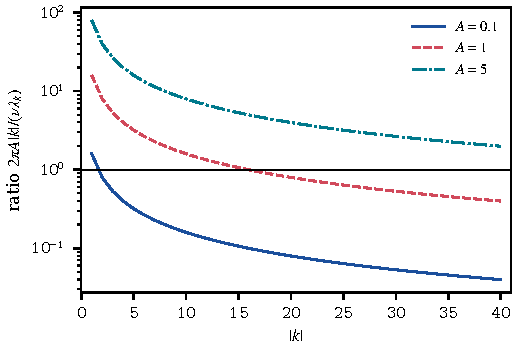
\includegraphics[width=0.75\textwidth]{mf_tg}
\caption{Ratio of advective coupling to viscous decay, $2\pi A|k|/(\nu\lambda_k)$ with $\lambda_k=4\pi^2|k|^2$ (the unit torus), for the linearized Navier Stokes equation about the Taylor Green vortex of amplitude $A$, $\nu=0.01$; the horizontal line marks one. Where the ratio exceeds one the nonlinear correction $\Kcal$ to the Stokes information operator matters; where it is small the Stokes formulas of Section~\ref{m:sec:heat} govern the posterior. The crossover scale grows linearly in $A/\nu$.}\label{m:fig:tg}
\end{figure}

\subsection{The sufficient statistic and the pipeline}

Definition~\ref{m:def:summary} specializes as follows. Given a preliminary estimate $\bar\theta_N$ from one half of the data (for Taylor Green, a few mode least squares fit of its early observations), compute, on the observations of the other half:
\begin{enumerate}[nosep]
\item the nonlinear forward solve $u_{\bar\theta_N}$ on $[0,T]$ by a pseudospectral method, and the residuals $r_i=Y_i-u_{\bar\theta_N}(t_i,x_i)$;
\item the adjoint linearized solve: $w$ solves, backward in time,
\[
\begin{split}
-\partial_sw+\nu Aw+{}&B[u_{\bar\theta_N},\cdot]^*w+B[\cdot,u_{\bar\theta_N}]^*w\\
&=\sum_ir_i\,\delta_{x_i}\delta_{t_i},\qquad w(T)=0,
\end{split}
\]
where the adjoints of the advection terms are, by Proposition~3.1(i) of Konen and Nickl~\cite{konennickl2026} and a direct computation, $B[u,\cdot]^*w=-B[u,w]$, which uses $\nabla\cdot u=0$ and periodicity, and $B[\cdot,u]^*w=P[(\nabla u)^\top w]$, in which $\nabla u$ is the Jacobian $(\nabla u)_{ij}=\partial_ju_i$, so that $\big((\nabla u)^\top w\big)_j=\sum_i w_i\partial_ju_i$; then $\I^*_{\bar\theta_N}r=w(0)$;
\item the application of $(F_N+\Sigma_0^{-1})^{-1}$, with $F_N$ the realized information of Remark~\ref{m:rem:reg}, by conjugate gradients (CG) preconditioned with the explicit Stokes inverse $2\nu(-\Delta)(\Id-S_{2T})^{-1}$ from \eqref{m:eq:fredholm}, each iteration costing one tangent solve and one adjoint solve.
\end{enumerate}
The output is \eqref{m:eq:regsummary}, the summary we compute (Remark~\ref{m:rem:reg}); with $(\I^*_{\bar\theta_N}\I_{\bar\theta_N})^{-1}$ in step 3 and $p_N$ applied to $w(0)$ before it, it is \eqref{m:eq:onestep} for one fold, and its average over the two folds, projected onto the first $J_N$ Stokes modes, is the summary $\hat S_N$ of Definition~\ref{m:def:summary}. Steps 1 and 2 are one gradient evaluation of 4DVar, and step 3 is a Gauss Newton solve. The GBC generator then learns the map from the summary to posterior draws, which by Remark~\ref{m:rem:affine} is asymptotically the identity plus the scale $T(\I^*\I)^{-1}/N$, whose diagonal is the Stokes scale of Table~\ref{m:tab:iota} corrected by the Taylor Green coupling at low $|k|$.

\subsubsection{What Konen Nickl's theorem says for this example} With $\alpha>12$, $\theta_0=u_{\rm TG}(0)$ smooth, and $T_0=0$: the posterior on $\theta$ is asymptotically $N(\tilde\theta_N,T(\I^*_{\theta_0}\I_{\theta_0})^{-1}/N)$ in $\Hds{-\sigma}$, $\sigma>9$; the posterior on $u_\theta(t)$ for $t\in[t_{\min},t_{\max}]$ is asymptotically the Gaussian field solving \eqref{m:eq:tangentgen} with initial datum from that law, at rate $1/\sqrt N$ in supremum norm; a credible band of posterior probability $1-\beta$ around $u_{\tilde\theta_N}$ has frequentist coverage $\to1-\beta$; and no estimator does better in local asymptotic minimax sense. The Taylor Green structure lets one see the covariance: it is the Stokes covariance on the diagonal, modified at $|k|\lesssim A/(2\pi\nu)$ on the unit torus (at $|k|\lesssim A/\nu$ on the $2\pi$ torus) by the nearest neighbor coupling, and the modification is a compact operator so it does not change the tightness range or the RKHS. For the advection functional $\Phi_t(u)=(u\cdot\nabla)u$ at time $t$, the delta method of Section~2.4 of Konen and Nickl~\cite{konennickl2026} gives a $\sqrt N$ Gaussian limit for $\Phi_t(u_{\tilde\theta_N})$, and for Taylor Green $\Phi_t(u_{\rm TG})$ is a gradient field, so the limit describes the fluctuation of the pressure gradient.

\subsubsection{The pipeline} The Navier Stokes pipeline is: pseudospectral simulations from a localized proposal (Step 1 of Algorithm~\ref{m:alg:gbc}, as amended in Algorithm~\ref{m:alg:loc}); per simulated data set, the summary \eqref{m:eq:regsummary} computed above; an identity skip quantile network with a learned scale (Step 2); evaluation at the observed summary (Step 3); forward simulation of the draws (Step 4), or by Corollary~\ref{m:cor:commute} simulation of the tangent equation from the Gaussian limit. With observations on $[T_0,T]$, $T_0>0$, Table~\ref{m:tab:iota} says which modes are lost; the pipeline is unchanged, and the scale learned in Step 2 becomes enormous for $|k|\gtrsim(\nu T_0)^{-1/2}$, which is correct.

\subsection{What survives a realistic design}\label{m:sec:designrobust}

The design in \eqref{m:eq:model} is $N$ points drawn independently and uniformly on $[0,T]\times\Omega$. Real observing systems are not that: they are fixed stations, satellite swaths on repeat orbits, radiosondes at synoptic hours, with errors correlated in space and between channels, and with observation operators, radiances or column integrals, that are not point evaluations.

\emph{Design robust.} Everything that holds for an arbitrary set of design points or depends on the design only through its information operator. Let $\varpi$ be any probability measure on $[0,T]\times\Omega$ and define $\langle h,\I^*_\varpi\I_\varpi h\rangle=\int|\I_\theta h|^2\,d\varpi$, which for the uniform design of \eqref{m:eq:model} is $T^{-1}\langle h,\I^*\I h\rangle$. Lemma~\ref{m:lem:adjoint}, Proposition~\ref{m:prop:linsuff}, Lemma~\ref{m:lem:exact} and Theorem~\ref{m:thm:gap} hold verbatim, and so does the first part of Theorem~\ref{m:thm:locbias}, the mean and variance \eqref{m:eq:varR} of the residual. The regularized summary of Remark~\ref{m:rem:reg} uses the realized information of the design actually drawn and needs no change, and Definition~\ref{m:def:summary} holds with $(\I^*_\varpi\I_\varpi)^{-1}$ in place of $T(\I^*\I)^{-1}$, given pilot estimators with the rates it asks for under $\varpi$. Theorem~\ref{m:thm:main} carries over once the Bernstein von Mises theorem and the conditions behind it are assumed to hold under $\varpi$ (Theorem~\ref{m:thm:nickl2} is proved for independent uniform times and points). Proposition~\ref{m:prop:radius} carries over once Conditions 2A to 2D hold with $\varpi$ in place of the uniform measure and the per coordinate form of Theorem~\ref{m:thm:locbias}, on which its term $\beta(c)$ rests, is available; that form needs the information operator to commute with the prior covariance. For the heat and Stokes equations a design that is uniform in space at each time, whatever the law of the times, keeps $\I^*_\varpi\I_\varpi$ diagonal in $(e_j)$, with the per mode information $\int e^{-2\nu\lambda_jt}\,d\varpi$ in place of $\iota_j$; under a design that is not uniform in space $\I^*_\varpi\I_\varpi$ is in general not diagonal. Correlated errors are equally harmless: with noise covariance $\Sigma_\varepsilon$ in place of $\varsigma^2\Id$, replace $\I^*\I$ by $\I^*\Sigma_\varepsilon^{-1}\I$ throughout and the adjoint statistic by $\I^*\Sigma_\varepsilon^{-1}r$, one extra linear solve. Observation operators that are not point evaluations are the same statement: if observation $i$ reports $\langle A_iu,\cdot\rangle$ rather than $u(t_i,x_i)$, the adjoint is driven by $\sum_ir_iA_i^*$ in place of $\sum_ir_i\delta_{X_i}$.

\emph{Not design robust.} Three things use the i.i.d. uniform design itself. Proposition~\ref{m:prop:gram} is a matrix Bernstein bound and needs independent summands, as do the second moment bounds on the whitened Gram matrix behind Propositions~\ref{m:prop:regheat} and~\ref{m:prop:regfixed}; under a correlated or deterministic design each must be replaced by a bound for dependent or fixed designs, and the concentration of $\Phi^\top\Phi$ on $N\,\diag(\iota_j)$ that Remark~\ref{m:rem:reg} warns about is exactly what degrades. The closed forms $\iota_j=\tfrac1T\int_0^Te^{-2\nu\lambda_jt}dt$ of \eqref{m:eq:iota} and the numbers in Table~\ref{m:tab:iota} are the uniform design values and change under any other $\varpi$; a fixed station network, for instance, samples $\Omega$ on a lattice and aliases modes above its Nyquist frequency, which no amount of data repairs. And the identification of $J_N$ with $N\delta_N^2$ presumes the law of large numbers (LLN) limit of the uniform design; under a design that never visits part of $\Omega$, the relevant dimension is set by the reachable subspace instead.

The practical reading is that the method transfers and the numbers do not. An implementer should recompute $\I^*_\varpi\I_\varpi$ for the observing system at hand rather than reuse $\iota_j$, and should expect Remark~\ref{m:rem:reg}'s regularized summary to matter more, not less, since a realistic design is further from its LLN limit than a uniform one. Every experiment reported in Section~\ref{m:sec:experiments}, the Navier Stokes run included, uses the uniform design of \eqref{m:eq:model}.
